\documentclass[portrait,final]{baposter}
%\documentclass[a4shrink,portrait,final]{baposter}
% Usa a4shrink for an a4 sized paper.

%\tracingstats=2

\usepackage{times}
\usepackage{calc}
\usepackage{graphicx}
\usepackage{amsmath} 
\usepackage{amssymb}
\usepackage{amsbsy} 
\usepackage{relsize}
\usepackage{multirow}
\usepackage{bm}
%\usepackage{natbib}

\usepackage{graphicx}   
\usepackage{multicol}

\usepackage{pgfbaselayers}
\pgfdeclarelayer{background}
\pgfdeclarelayer{foreground}
\pgfsetlayers{background,main,foreground}
\usetikzlibrary{shadows}

\usepackage{helvet}
%\usepackage{bookman}
\usepackage{palatino}


\selectcolormodel{cmyk}


\begin{document}
\definecolor{lightersilver}{cmyk}{0,0,0,0.1}
\definecolor{silver}{cmyk}{0,0,0,0.3}
\definecolor{darksilver}{cmyk}{0,0,0,0.4}
\definecolor{yellow}{cmyk}{0,0,0.9,0.0}
\definecolor{reddishyellow}{cmyk}{0,0.22,1.0,0.0}
\definecolor{black}{cmyk}{0,0,0.0,1.0}
\definecolor{darkYellow}{cmyk}{0,0,1.0,0.5}
\definecolor{darkSilver}{cmyk}{0,0,0,0.1}
%\definecolor{darkSilver}{cmyk}{0,0,0,0.1}
\definecolor{green}{rgb}{0.5,0.9,0.0}
\definecolor{darkgreen}{rgb}{0,0.6,0}


\definecolor{lightyellow}{cmyk}{0,0,0.4,0.0}
\definecolor{lighteryellow}{cmyk}{0,0,0.1,0.0}
\definecolor{lightestyellow}{cmyk}{0,0,0.05,0.0}

\newcommand{\bs}[1]{\boldsymbol{#1}}

\begin{poster}%
{
grid=no,
colspacing=0.7em,
bgColorOne=white,%lightersilver, 
bgColorTwo=white,%lightersilver,
borderColor=darkgreen,%reddishyellow, 
headerColorOne=green,%yellow,
headerColorTwo=darkgreen,%reddishyellow, 
headerFontColor=black,
boxColorOne=lightersilver,
boxColorTwo=lighteryellow,
textborder=rounded,
eyecatcher=yes,
headerborder=open,
headerheight=0.09\textheight, 
headershape=rounded,
headershade=shade-tb,
headerfont=\Large\textbf, %Sans Serif 
boxshade=plain, 
background=plain,
linewidth=2pt
}
  % Eye Catcher must be on to center the rest
{\includegraphics[height=1.9cm]{Arabidopsis_thaliana_inflorescenciasB.jpg}\hspace{.2cm} 
} 
{\huge MSMS\\ \LARGE Simulating the patterns of molecular evolution}
{\sc \hspace{1cm} Mathematics and BioSciences Group
\newline {\small Greg Ewing, Ines Hellmann, Christian Huber, Joachim Hermisson}}
{
\begin{minipage}{0.2625\textwidth}
%\begin{center}

\includegraphics[height=1cm]{uni_logo_farbe_01.pdf}
\newline
\includegraphics[height=1cm]{mfpl_logo3d_transparent.png}
%\end{center}
\end{minipage}
}   
%%%%%%%%%%%%%%%%%%%%%%%%%%%%%%%%%%%%%%%%%%%%%%%%%%%%%%%%%%%%%%%%%%%%%%%%%%%%%%
%%% Now define the boxes that make up the poster
%%%---------------------------------------------------------------------------
%%% Each box has a name and can be placed absolutely or relatively.
%%% The only inconvenience is that you can only specify a relative position 
%%% towards an already declared box. So if you have a box attached to the 
%%% bottom, one to the top and a third one which should be in between, you 
%%% have to specify the top and bottom boxes before you specify the middle 
%%% box.
%%%%%%%%%%%%%%%%%%%%%%%%%%%%%%%%%%%%%%%%%%%%%%%%%%%%%%%%%%%%%%%%%%%%%%%%%%%%%%
 
\headerbox{Abstract}{name=abstract,column=0,row=0}{
We have implemented a coalescent simulation program for a structured population
with selection at a single diploid locus with high performance called {\it
msms}\cite{ewing2010}. This program can be used to study the patterns of molecular
evolution under a wide range of different scenarios. One such scenario is the study of Arabidopsis throughout
Europe. Arabidopsis recolonized Europe after glacial retreat at the end of the
last ice age. Detecting adaptive selection from the wide range of climates is
complicated by the recolonization patterns which can confound tests of selective
sweeps. By using {\it msms}, we can study how current tests perform as well as
develop new tests.
  \vspace{0.4em}
}

\headerbox{Power and False Positives}{name=power,row=0,span=1,column=2}{

\subsection*{How strong does a selective sweep need to be before we can detect
it? What is the false positive rate?}
Various tests have been devised for detecting selective sweeps. Choosing a cutoff
value for a statistic generally involves a trade off between false positives and
power (true positive).
\vspace{-.25cm}
\begin{center} 
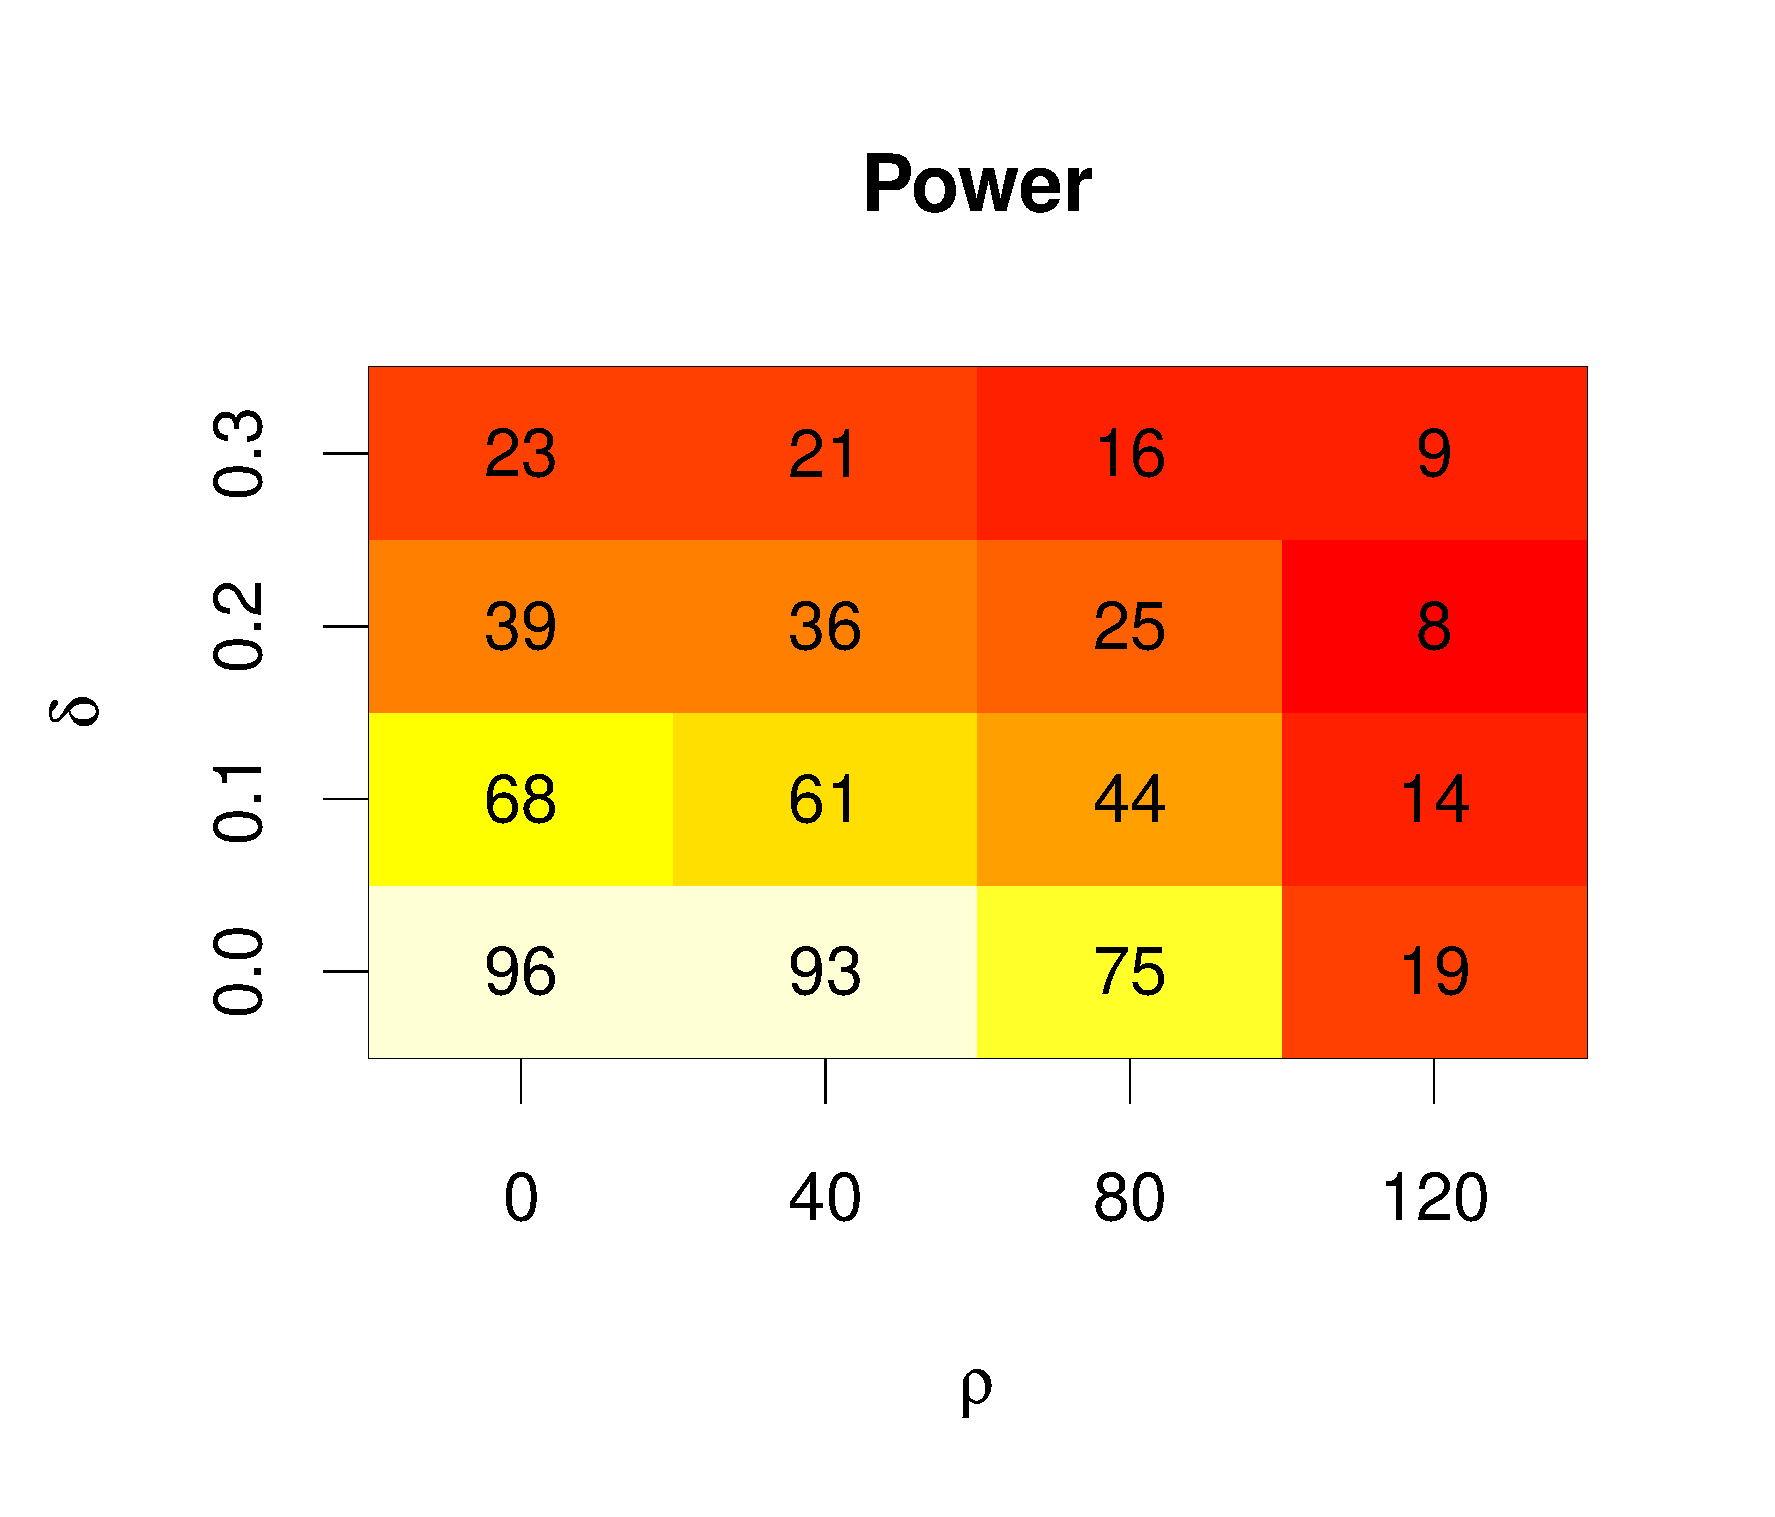
\includegraphics[width=1.05\textwidth]{power.pdf}
\end{center}
\vspace{-.25cm}
In the above figure, we see the power of a simple Tajima's D test on a single
deme without any population growth. $\delta$ denotes the time since the sweep in
$4N_e$ generations and $\rho=2Nr$ is the between locus recombination distance. The
within locus recombination is $\rho_{in}=10$
\vspace{-.25cm}
\begin{center}
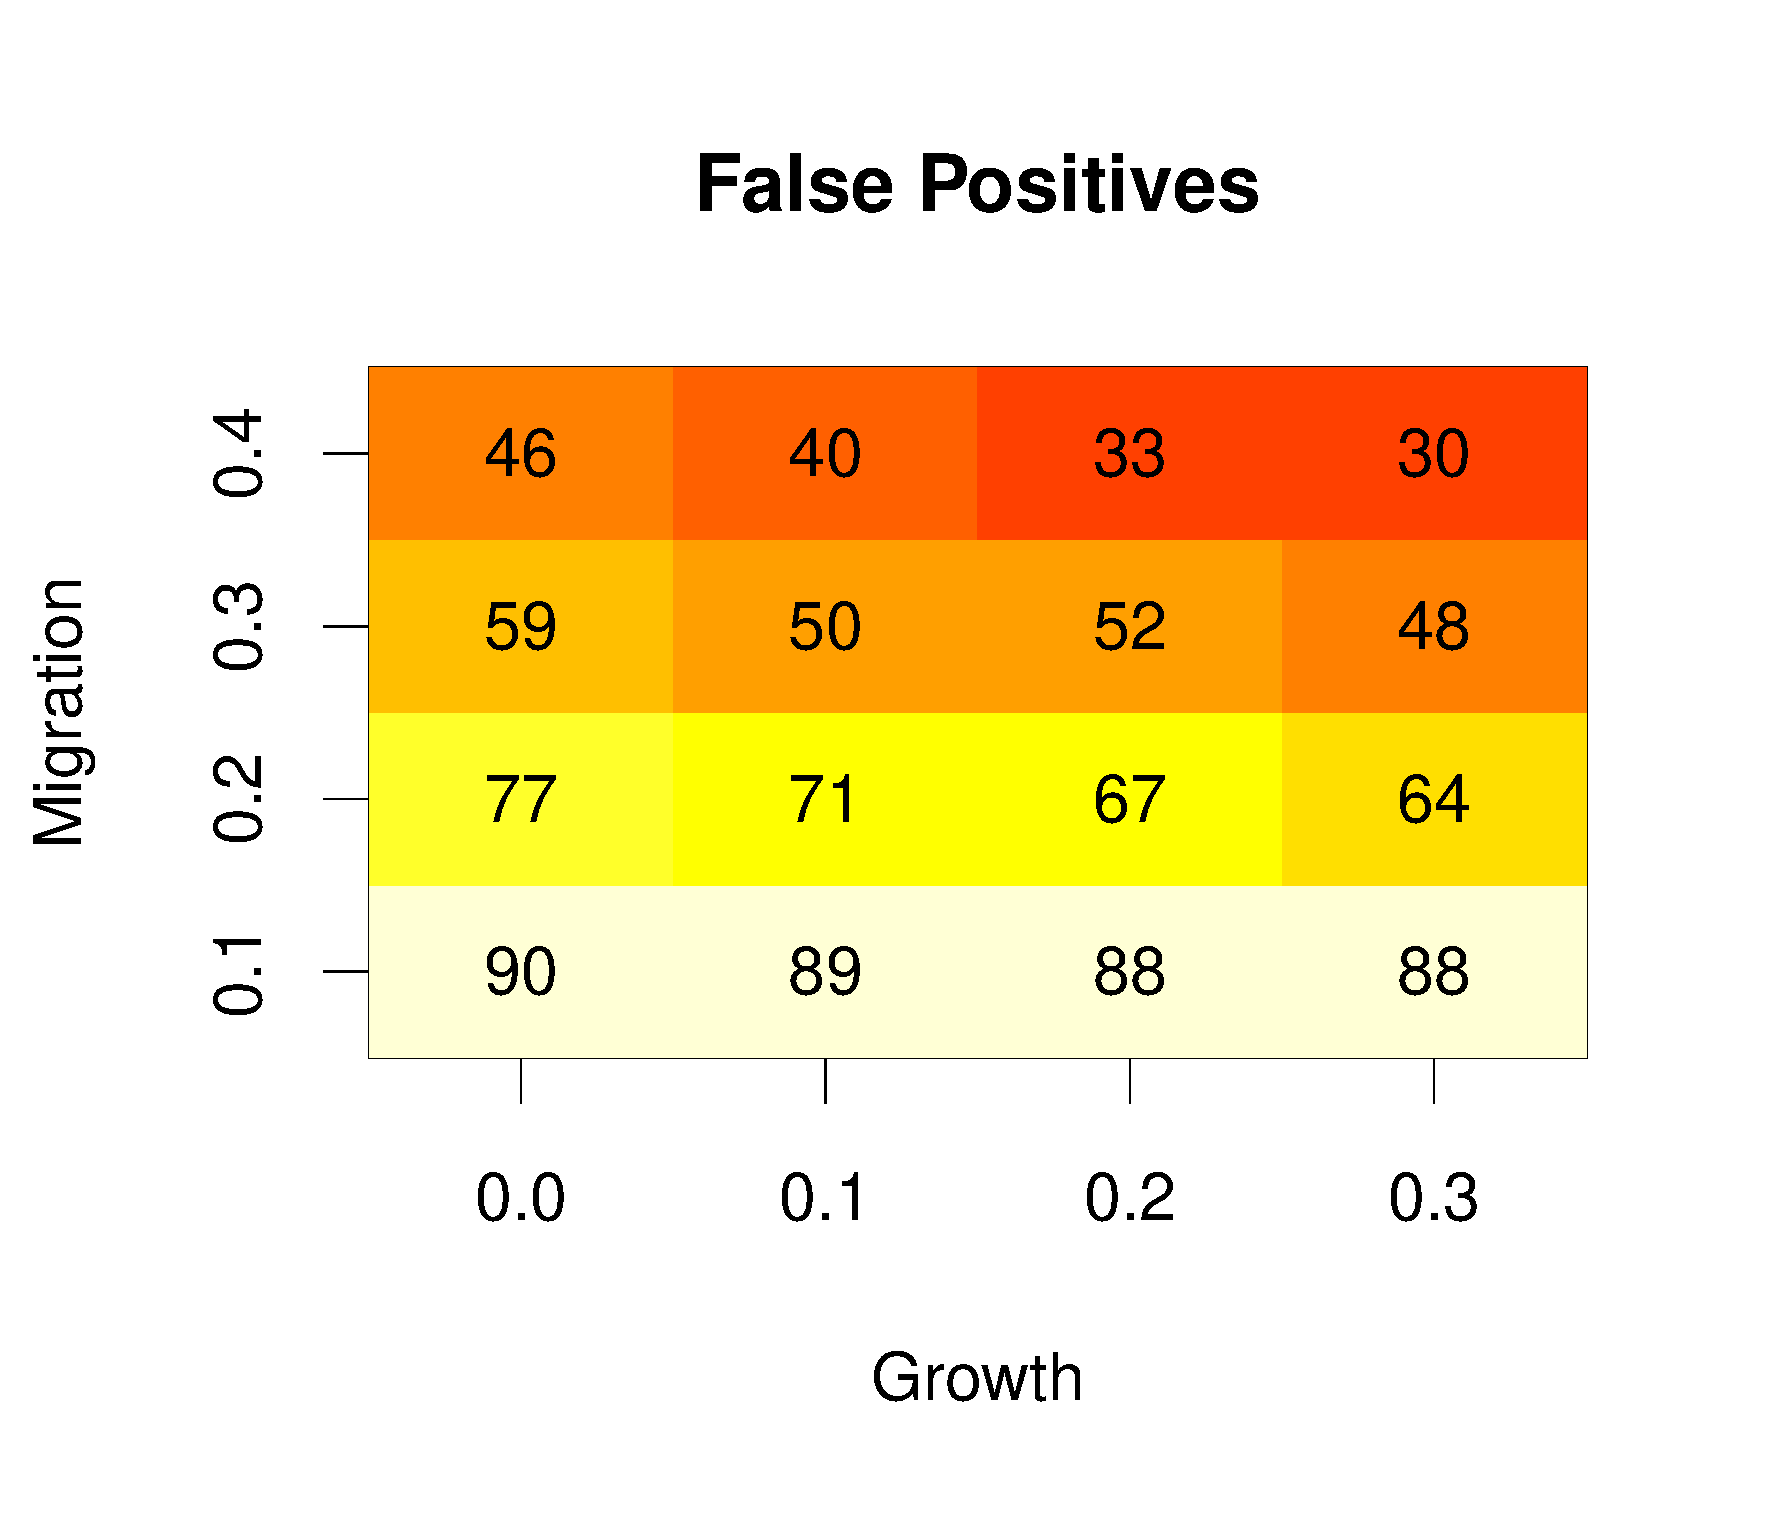
\includegraphics[width=1.05\textwidth]{false.pdf}
\end{center}
\vspace{-.25cm}
However if there is population structure or population size change, the
false positive rate becomes very large as the above figure shows. Here, we have
just 2 demes with symmetric population growth and migration. From this it is
clear that tests should be conditioned on the demography, or be insensitive to
it. 
\vspace{.5em}
}

% \headerbox{{ msmsABC}}{name=abc,column=2,below=power}{
% 
% The ability to simulate all kinds of selective scenarios efficiently opens the possibility to 
% estimate selection parameters via Approximate Bayesian Computation (ABC). 
% %{\it msmsABC} is  to be compatible with the ABC toolbox from
% %the CMPG lab at the University of Bern.
% 
% \mbox{
% \begin{tikzpicture}[scale=.5]
% \draw (-1.5,0) node[anchor=north west]
% {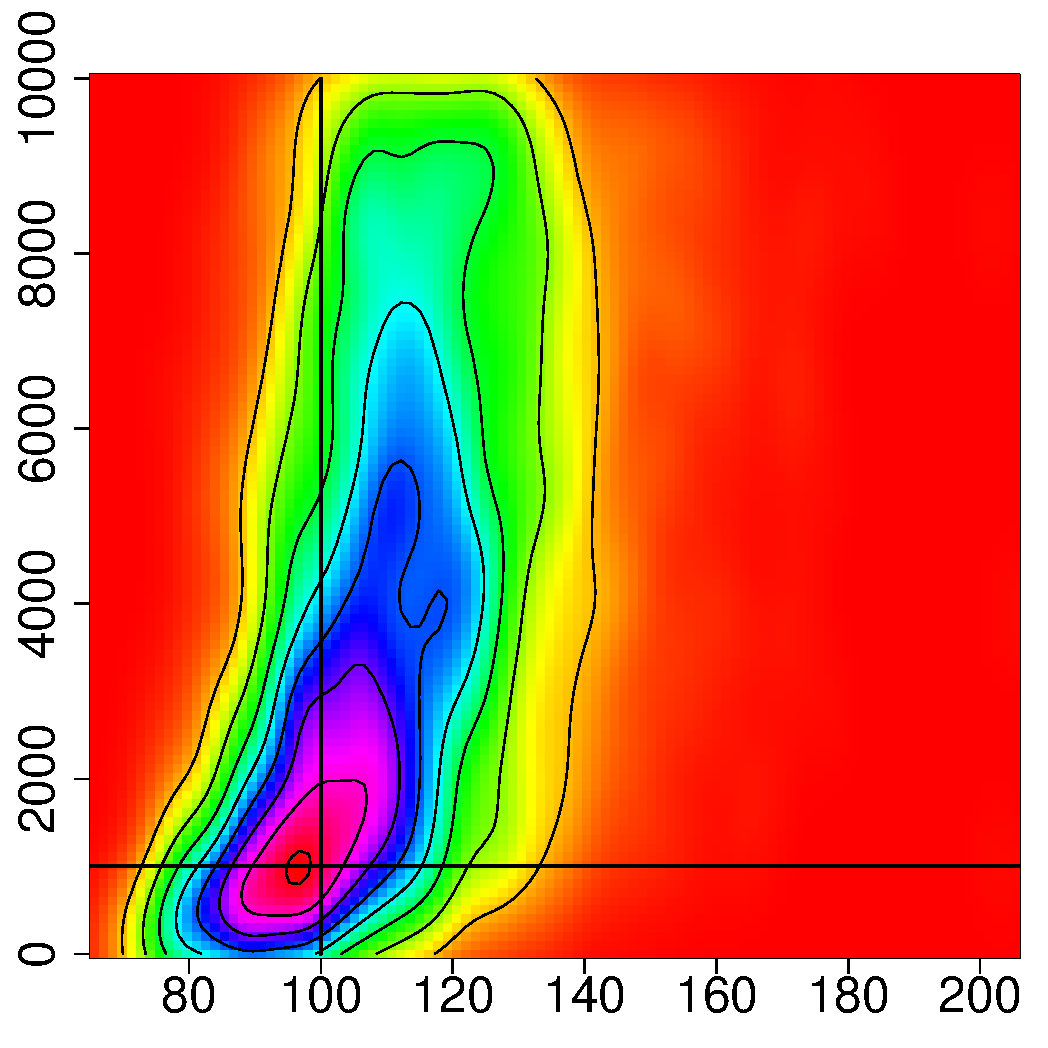
\includegraphics[width=0.4\textwidth]{2dAlphaThetaL.pdf}}
% %(1.5,0.1) node[above] 
% %{\bfseries Estimation of some selection parameters}
% (-1.7,-2.75) node[left] {\large $\bs\alpha$}
% (1.5,-6) node[below] {\large $\bs\theta$};
% \end{tikzpicture}\quad 
% \begin{tikzpicture}[scale=0.5]
% \draw (-1.5,0) node[anchor=north west]
% {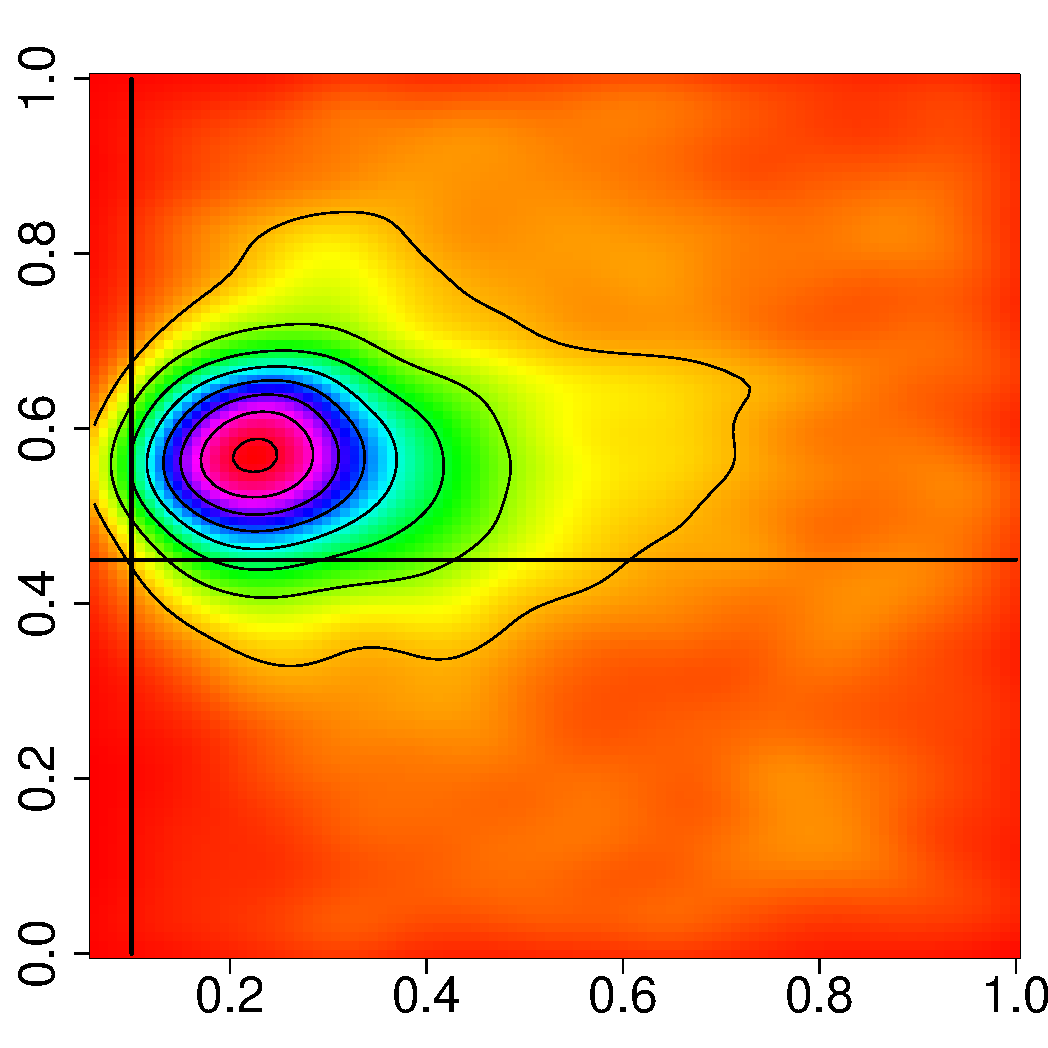
\includegraphics[width=0.4\textwidth]{2dPosTimeL.pdf}}  
% %(1.5,0) node[above] 
% %{\bfseries Position of Selected Site and Fixation Time}
% (-1.9,-1.5) node[left,rotate=90] {\bfseries Position}
% (1.5,-6.0) node[below] {\bfseries Fixation Time};
% \end{tikzpicture}
% }
% 
% \vspace{0.5em}
% 
% The figures show successfully estimation of the mutation parameter $\theta$ and
% selection strength $\alpha$. However currently poor estimation of the position
% of the selected locus and time of fixation. However better performance is
% expected with iEHH type statistics. 
% \vspace{.5em}
% }
 




\headerbox{Simulation Method}{name=sims,below=abstract,column=0}{

{\it MSMS}\cite{ewing2010} uses an infinite sites mutation model and locus
model.
\vspace{.1cm}

\includegraphics[width=1\textwidth]{locus.pdf}

Simulations are carried out in the following steps:
\begin{enumerate}
  \item A forward pass simulates selection with drift. The
  result is the frequency of the selected allele over time for each deme.
  \item The coalescent is then simulated in the pastward direction {\em
  conditional} on the frequency of the selected locus.
  \item Neutral mutations are added to the ancestral recombination graph.
\end{enumerate}
To sample the coalescent conditionally on frequency,  we assume discrete generations 
during the selected phase. Two lineages can only be recombinant
descendants of a parent if they share the allele at the selected locus. Therefore the
effective population size of the selected allele is scaled by the frequency.
All other events are affected similarly. 
\vspace{0.4em}
}

\headerbox{Performance: {\it msms } vs. {\it ms}}
{name=speed,below=sims,column=0}{

\begin{tikzpicture}
\draw (-1.5,0.4) node[anchor=north west]
{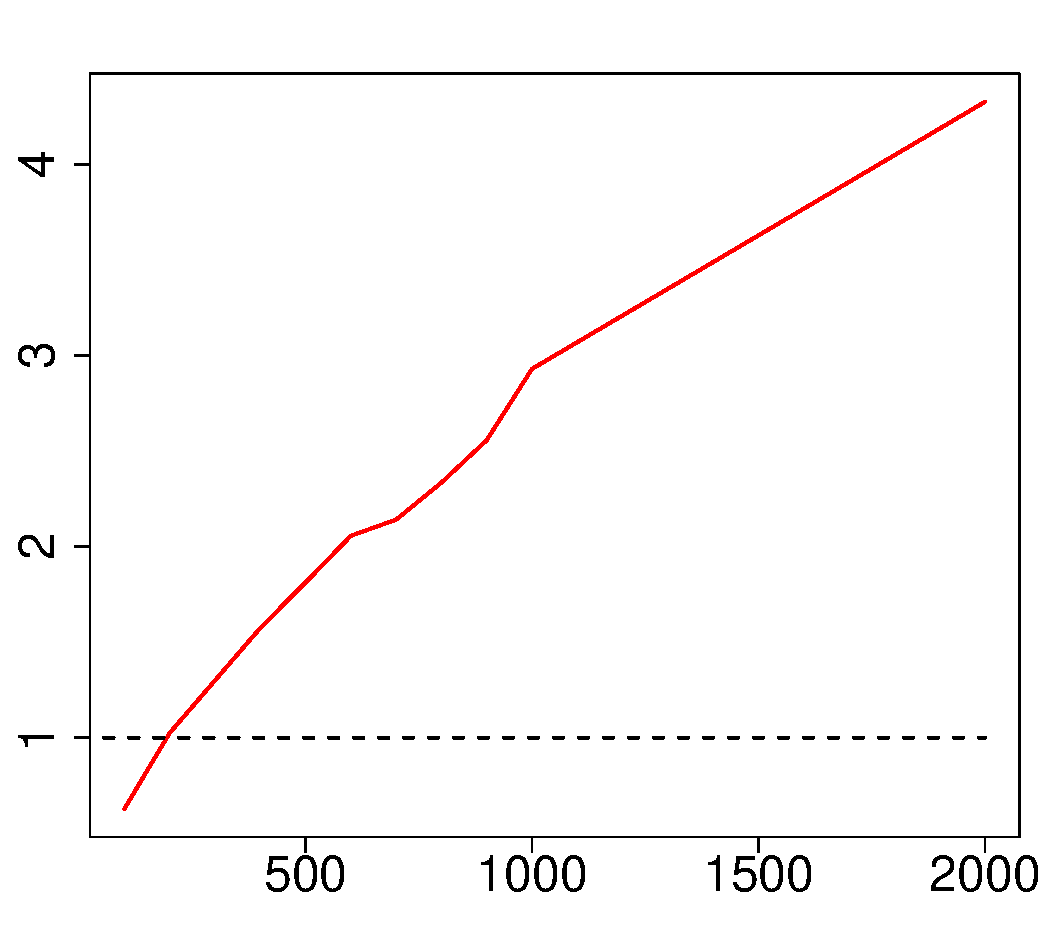
\includegraphics[width=0.8\textwidth]{fastL.pdf}}
(1.5,0) node[above] 
{\bfseries Speedup Ratio of {\it msms} vrs {\it ms}}
(-1.7,-1) node[left,rotate=90] {\bfseries Speedup Factor}
(1.5,-4.8) node[below] {\bfseries Recombination Rate $\bs\rho$};
\end{tikzpicture}

The figure shows the computing speed of {\it msms} without selection compared to
{\sc ms} on a standard desktop PC:  AMD64 X2 Dual Core Processor 6000+, using Sun
Java 1.6u18 64bit and gcc 4.2.3.
{\it msms} is faster than {\sc ms} with intermediate to high
recombination. The command line used was:

{\tt ms 50 1000 -t 100 -r $\rho$ 10000}

\vspace{0.4em}
}



\headerbox{Sweeps in Arabidopsis?}
{name=data,column=1,row=0,span=1}{ 
\begin{center}
\begin{tikzpicture}
\draw (0,0) node[anchor=north west] 
{\includegraphics[width=\textwidth]{colourMap.pdf}}; 
%(0,-20) node {wtf};
\end{tikzpicture}
\end{center}
\vspace{-.3cm}
In collaboration with GMI (Magnus Nordborg's group) we will be analyzing a
subset of the 1001 genomes project. 
\begin{center}
 \section*{The Data}
\end{center}
\begin{itemize}
  \item 106 full Arabidopsis genomes from Sweden.
  \item Phenotypes and GPS positions.
  \item Strong populations structure: recolonization from glacial refuges.
\end{itemize}

\begin{center}
\section*{Questions}
\end{center}
\begin{itemize}
  \item What is the impact of population structure on genomic polymorphism data?
  \item Can we separate signatures of selection (selective sweeps) from
dispersive effects and estimate parameters for selection and demography?
  \item Can we detect genes underlying local adaptation?
\end{itemize}

\begin{center}
\section*{Approach}
\end{center}
\begin{itemize}
  \item We can model many deme models quickly with {\it msms}.
  \item Can study behavior of ideal models, while comparing with real data. 
  \item Develop tests that condition on demography or are insensitive to it. 
\end{itemize}

} 
\headerbox{Conclusion}
 {name=theend,below=power,span=1,column=2,bottomaligned=speed}{
 \large
 {\it MSMS}\cite{ewing2010} is a powerful coalescent simulator with selection at
 a single locus. A wide range of applications are possible with the combination
 of flexibility and speed that {\it msms} provides.  A specific application
 is an Arabidopsis data set throughout Sweden, where  separating population
 structure and local adaptation are challenging problems to detecting selective 
 sweeps. 
 \vspace{.5em}
 }

\headerbox{\normalsize Citations and Acknowledgments}
{name=cite,below=data,column=1,bottomaligned=speed} { 
\small 

Funding from the DFG and the WWTF is gratefully acknowledged. Thanks also to
Peter Pfaffelhuber, Cornelia Borck, Ines Hellmann, Pleuni Pennings and Jayne
Ewing.

\vspace{-1.2cm}
\bibliographystyle{Science}
\renewcommand\refname{}
\bibliography{Bio}
}


\end{poster}% 
\end{document}
